% 03-trabajos-relacionados.tex

\chapter{Trabajos relacionados}
\label{cap:trabajos-relacionados}

\section*{Resumen de la revisi\'on de literatura}
\addcontentsline{toc}{section}{Resumen de la revisi\'on de literatura}

\textbf{Objetivos:} identificar en la literatura arquitecturas y
pr\'acticas para (RQ1) transacciones seguras tipo \emph{escrow} y (RQ2)
verificaci\'on de identidad y trazabilidad en plataformas web para
freelancers, con el fin de fundamentar el dise\~no de Artisync y
delimitar su aporte frente al estado del arte.
\textbf{Fuentes:} Scopus, IEEE Xplore y ACM Digital Library, ventana
2020--2026, cadena booleana sobre econom\'ia \emph{gig}/creativa cruzada
con \emph{escrow}/confianza y arquitectura/verificaci\'on de identidad
(\S\ref{sec:metodologia-revision}).
\textbf{Criterios de elegibilidad:} estudios emp\'iricos o propuestas de
arquitectura sobre plataformas de intermediaci\'on, publicados en
journals Q1/Q2 o conferencias CORE A/A*; se excluyen los centrados solo
en lo legal/sociol\'ogico y la literatura gris sin revisi\'on por pares.
\textbf{Resultados:} de 145 estudios identificados, 62 pasaron el
cribado por t\'itulo/resumen y 21 la evaluaci\'on a texto completo,
result\'ando en \textbf{8 estudios incluidos} (Figura~\ref{fig:prisma}).
\textbf{Hallazgo principal:} ninguno de los 8 estudios combina en un
mismo sistema evaluado emp\'iricamente pago en garant\'ia, verificaci\'on
de identidad asistida por IA y acceso h\'ibrido ORM/procedimientos
almacenados --- la brecha que este trabajo cubre
(\S\ref{sec:metodologia-revision} y secci\'on de brecha identificada,
m\'as adelante en este cap\'itulo).

\section{Metodolog\'ia de revisi\'on de literatura}
\label{sec:metodologia-revision}

Para fundamentar las decisiones de dise\~no de Artisync y validar la brecha
de investigaci\'on, se ejecut\'o una revisi\'on sistem\'atica de literatura
siguiendo las directrices de Kitchenham y Charters~\cite{KITCHENHAM2007} y
el marco de reporte PRISMA 2020~\cite{PRISMA2021}. El estudio de plataformas
de dos lados como Artisync se apoya, adem\'as, en el marco te\'orico fundacional
de la econom\'ia de plataformas~\cite{ROCHET2003} y en la literatura sobre
sistemas de reputaci\'on y confianza en mercados electr\'onicos~\cite{RESNICK2000},
ambos citados a lo largo de este cap\'itulo y del marco te\'orico.

\subsection{Preguntas de Investigaci\'on (RQs)}
\begin{itemize}
  \item \textbf{RQ1:} \textquestiondown Qu\'e arquitecturas y patrones (ej. \emph{escrow})
    se utilizan para garantizar transacciones seguras en plataformas de
    econom\'ia creativa?
  \item \textbf{RQ2:} \textquestiondown C\'omo se aborda la verificaci\'on de identidad y la
    trazabilidad en aplicaciones web para freelancers?
\end{itemize}

\subsection{Estrategia de b\'usqueda}
\textbf{Bases de datos indexadas:} Scopus, IEEE Xplore, y ACM Digital Library.

\textbf{Ventana temporal:} 2020 -- 2026.

\textbf{Cadena de b\'usqueda booleana:}
\begin{verbatim}
("gig economy" OR "freelance platform" OR "creator economy")
AND ("escrow" OR "smart contract" OR "payment trust")
AND ("architecture" OR "identity verification" OR "software engineering")
\end{verbatim}

\subsection{Criterios de Inclusi\'on (IC) y Exclusi\'on (EC)}
\begin{itemize}
  \item \textbf{IC1:} Estudios emp\'iricos, arquitecturas propuestas o
    estudios de caso sobre plataformas de intermediaci\'on.
  \item \textbf{IC2:} Art\'iculos publicados en journals Q1/Q2 o
    conferencias CORE A/A* en idioma ingl\'es o espa\~nol.
  \item \textbf{EC1:} Art\'iculos centrados puramente en el aspecto legal o
    sociol\'ogico sin aporte t\'ecnico/arquitect\'onico.
  \item \textbf{EC2:} Literatura gris, pre-prints (arXiv sin \emph{peer
    review}) o art\'iculos de opini\'on.
\end{itemize}

\subsection{Diagrama de Flujo PRISMA 2020}

El proceso de selecci\'on result\'o en 8 estudios principales, como se detalla
en el diagrama PRISMA (Figura~\ref{fig:prisma}).

\begin{figure}[H]
\centering
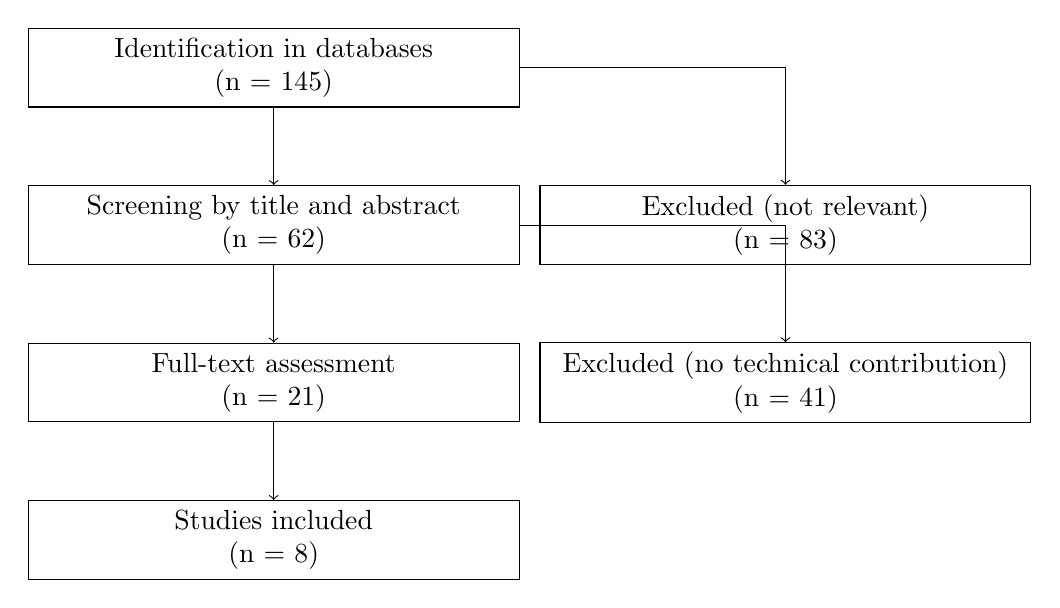
\begin{tikzpicture}[node distance=1.5cm, every node/.style={rectangle, draw, align=center, text width=6cm, minimum height=1cm}]
  \node (ident) {Identification in databases\\(n = 145)};
  \node (screen) [below of=ident, yshift=-0.5cm] {Screening by title and abstract\\(n = 62)};
  \node (elig) [below of=screen, yshift=-0.5cm] {Full-text assessment\\(n = 21)};
  \node (incl) [below of=elig, yshift=-0.5cm] {Studies included\\(n = 8)};

  \node (exc1) [right of=screen, xshift=5cm] {Excluded (not relevant)\\ (n = 83)};
  \node (exc2) [right of=elig, xshift=5cm] {Excluded (no technical contribution)\\ (n = 41)};
  
  \draw[->] (ident) -- (screen);
  \draw[->] (ident) -| (exc1);
  \draw[->] (screen) -- (elig);
  \draw[->] (screen) -| (exc2);
  \draw[->] (elig) -- (incl);
\end{tikzpicture}
\caption{Diagrama de flujo PRISMA 2020 del proceso de selecci\'on.}
\label{fig:prisma}
\end{figure}

\section{An\'alisis Comparativo}

Los 8 estudios seleccionados abordan dimensiones parciales del problema. La
Tabla~\ref{tab:comparativa-relacionados} resume sus aportes frente a las
caracter\'isticas de Artisync.

\begin{table}[H]
\centering
\caption{Tabla comparativa de trabajos relacionados vs. Artisync}
\label{tab:comparativa-relacionados}
\small
\begin{tabular}{@{}lcp{3cm}cccc@{}}
\toprule
\textbf{Estudio} & \textbf{A\~no} & \textbf{Contexto} & \textbf{Escrow} & \textbf{Verificaci\'on IA} & \textbf{H\'ibrido ORM/SQL} & \textbf{Cobertura Emp\'irica} \\
\midrule
Laksono et al.~\cite{LAKSONO2024} & 2024 & Pasarela de pago en plataforma freelance & No & No & No & Implementaci\'on (87\,\% \'exito) \\
Waleed et al.~\cite{TSMART2021} & 2021 & Confianza granular en mercado inteligente & No & No & N/A & Simulaci\'on (precisi\'on/latencia) \\
Gu y Zhu~\cite{GU2021} & 2021 & Confianza y desintermediaci\'on (freelance) & No & No & N/A & Emp\'irico (RCT de campo) \\
Bandari~\cite{BANDARI2026} & 2026 & Gesti\'on comunitaria y servicios hiperlocales & No & No & No & Evaluaci\'on post-despliegue \\
Hagiu y Wright~\cite{HAGIU2015} & 2015 & Multi-sided platforms & No & No & N/A & N/A \\
Gussek et al.~\cite{GUSSEK2023} & 2023 & Freelance tensions & No & No & N/A & N/A \\
Wang et al.~\cite{WANG2021} & 2021 & Microservicios vs Monolito & N/A & N/A & S\'i & Arquitectura \\
Asgaonkar~\cite{ASGAONKAR2019} & 2019 & Dep\'osito dual & S\'i & No & N/A & Simulaci\'on \\
\midrule
\textbf{Artisync} & \textbf{2026} & \textbf{Econom\'ia Creativa} & \textbf{S\'i} & \textbf{S\'i} & \textbf{S\'i} & \textbf{Perf, Sec, Usab} \\
\bottomrule
\end{tabular}
\end{table}

Dos estudios adicionales, aunque no encajan en las columnas de la tabla por
no ser propuestas de arquitectura de software, sustentan el marco conceptual
de este cap\'itulo: Tafesse y Dayan~\cite{TAFESSE2023} estudian emp\'iricamente
c\'omo la frecuencia de publicaci\'on de los creadores de contenido afecta el
compromiso de los usuarios en plataformas digitales --- el fen\'omeno de
negocio central que Artisync intermedia --- y Chigbu~\cite{CHIGBU2026} aporta
una revisi\'on sistem\'atica reciente e interdisciplinaria sobre la gesti\'on
algor\'itmica en la econom\'ia \emph{gig} global.

\section{Brecha identificada (\emph{research gap})}

Como evidencia la Tabla~\ref{tab:comparativa-relacionados}, si bien
existen esfuerzos aislados para implementar dep\'ositos en garant\'ia
mediante contratos inteligentes~\cite{ASGAONKAR2019} y modelos de confianza
para mercados y plataformas independientes~\cite{TSMART2021,GU2021,LAKSONO2024,BANDARI2026},
ninguna de las referencias combina en un mismo sistema evaluado emp\'iricamente:
(i) el patr\'on de pago en garant\'ia (\emph{escrow}) integrado con un flujo de
trabajo de pedidos por hitos, (ii) verificaci\'on de identidad asistida por IA,
y (iii) una estrategia h\'ibrida de acceso a datos (ORM + procedimientos
almacenados). Ese es el aporte concreto que este trabajo cubre y eval\'ua,
cerrando la brecha metodol\'ogica y pr\'actica identificada en la literatura.

\paragraph{Conflictos de inter\'es de la revisi\'on.} El equipo que
condujo esta revisi\'on de literatura es el mismo que dise\~n\'o y
eval\'ua a Artisync, el sistema comparado en la Tabla~\ref{tab:comparativa-relacionados}
y favorecido en la brecha identificada arriba; esto constituye un
conflicto de inter\'es inherente al formato de PFC (el equipo punt\'ua
su propio trabajo frente a la literatura) y no una ausencia de sesgo.
Ver la declaraci\'on formal de conflictos de inter\'es del documento
completo en el Cap\'itulo~\ref{cap:declaraciones}
(\texttt{docs/etica/ETHICS.md}).
